% !TEX root =  ../conclusions.tex
\section{Conclusions}

% What are your main conclusions from these results?
% This section should lead from the Results into the Improvements.
% Describe how you will improve our application based on your results. What changes will you make, and why? What would it look like before and after? Why is the improved version better? Motivate your choices using the heuristics and your results.
% The conclusion of this section should show your final GUI design.
% Note that this report is only about the design, so it is not necessary to already show the finished improved implementation.

Our main conclusion from these results is that the system largely fails on two fronts - Visibility of System Status and Error Recovery (principles \#1 and \#9, as detailed by Nielsen), with less pressing matters regarding the visual aspect. A number of interface elements that suggested certain functionalities that were at the time not yet implemented was also remarked. 

Taking these points to heart, the main improvements, whose necessity arises as evident, are the following:
\begin{itemize}
    \item Replace standard error messages with more user-friendly popups, or forgo popups entirely in favour of highlighting the error within the same screen.
    \item Clearly show the status of the user (admin or not).
    \item Add cancel buttons to the Add Card and Settings scenes.
    \item Use restrictions to prevent errors, such as a character limit on certain text fields, date-time and location input validation.
    \item Polish the visual aspect of the app, making sure the full-screen behaviour is not distracting, and ensuring visual consistency across the entire application. 
\end{itemize}

Not all the issues found during the evaluation will be translated into planned Improvements. For instance, some of the issues were caused by bugs or features that were already planned to be implemented, so this does not change the course of development. Other issues were a matter of personal preference, such as the colour scheme - this could be changed, or the option to let a user customise the appearance of the application could be added, but the team does not see it as a priority. 

After the improvements detailed in this section have been made, the product is expected to be much more easy to use for users that, for instance, might not know what an IP address or a hash code (the board key) is. The app is also expected to be significantly more forgiving to errors the user might cause. This is significantly more in line with the aforementioned Usability Heuristics.

\begin{figure}
    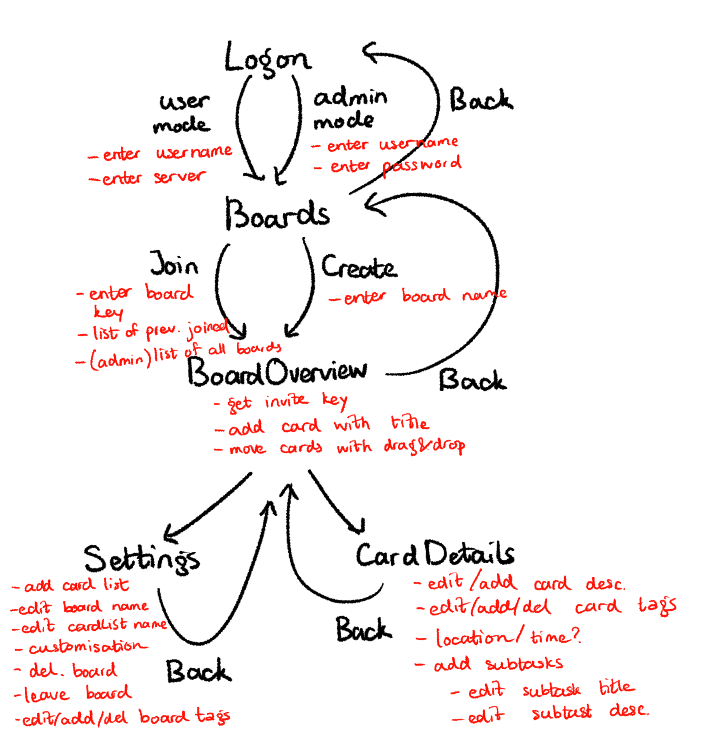
\includegraphics{mocks/hue_mock_flow.png}
    \caption{A "sitemap" of the application.}
\end{figure}

\begin{figure}
    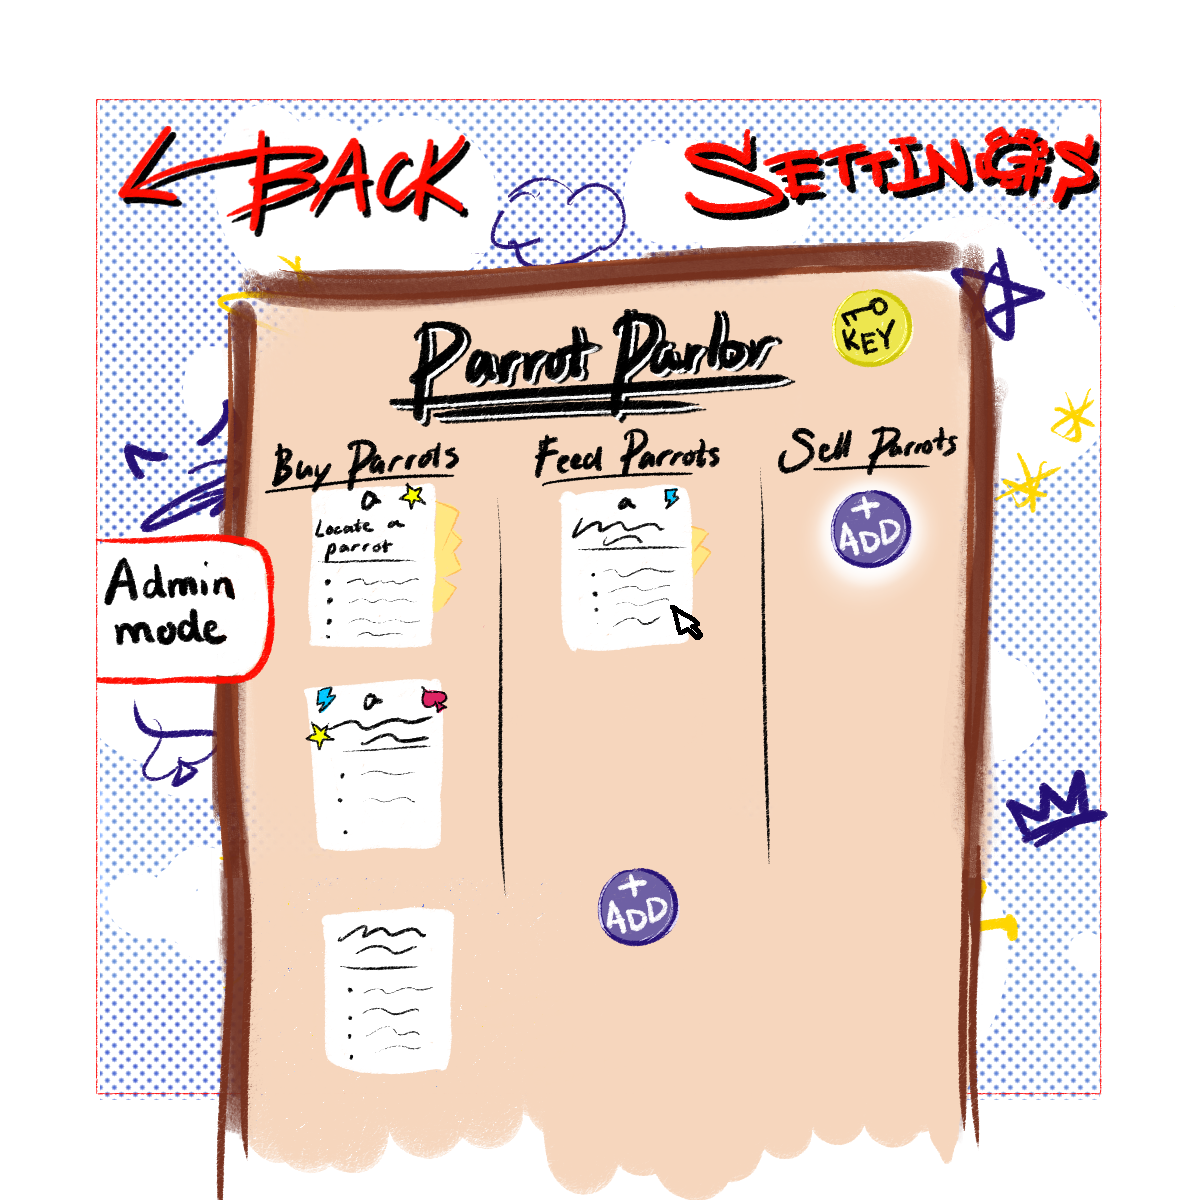
\includegraphics{mocks/hue_mock_board_overview.png}
    \caption{The board overview screen.}
\end{figure}
\begin{figure}
    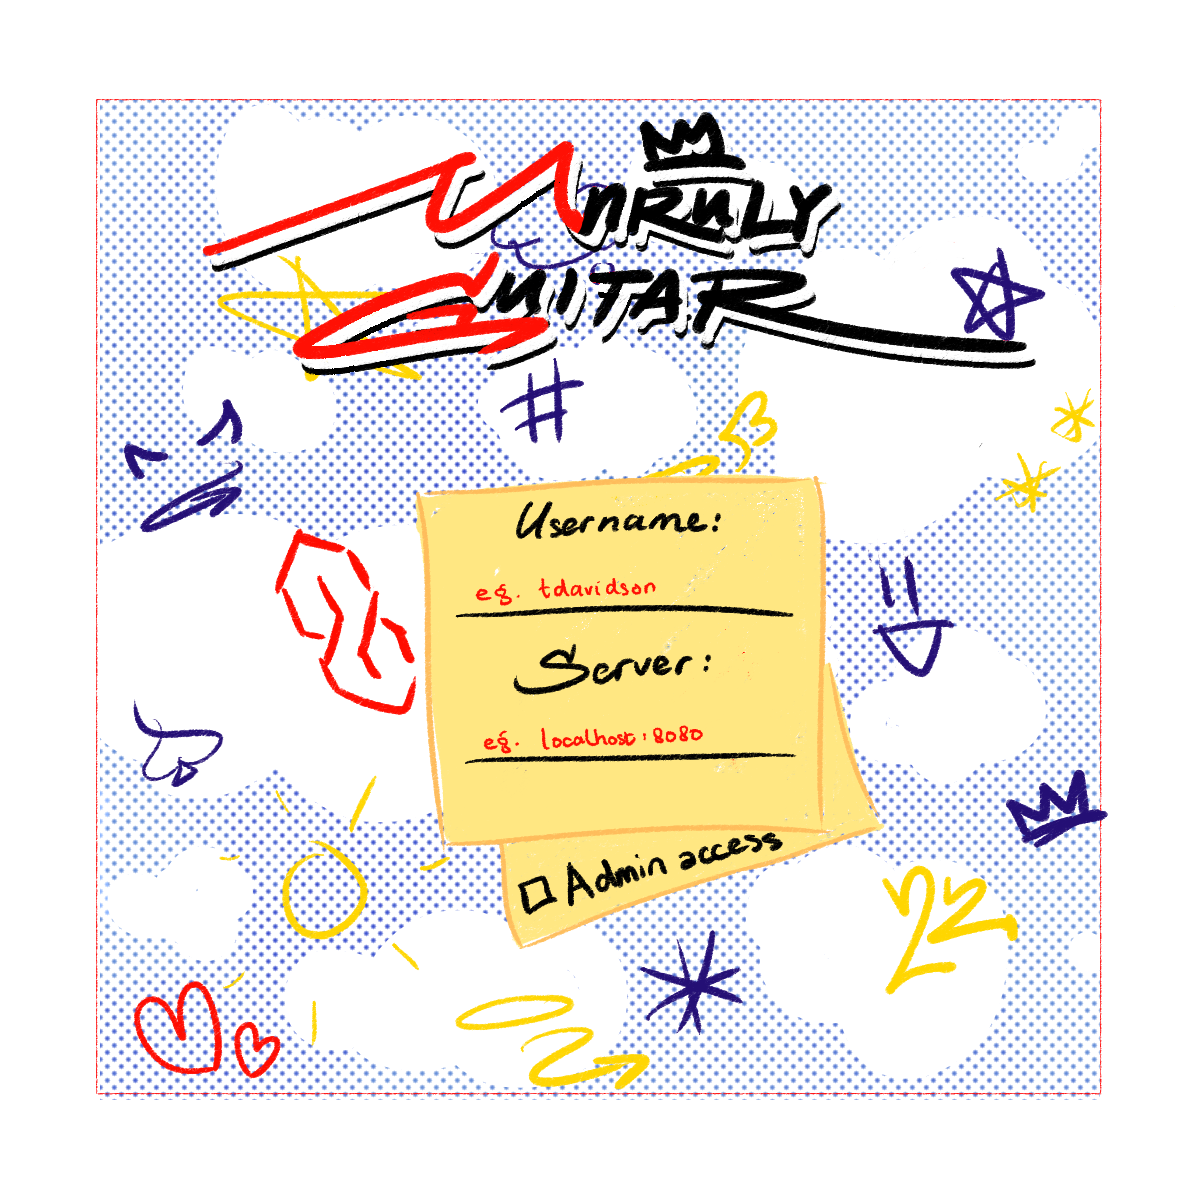
\includegraphics{mocks/hue_mock_logon.png}
    \caption{The logon screen.}
\end{figure}
\begin{figure}
    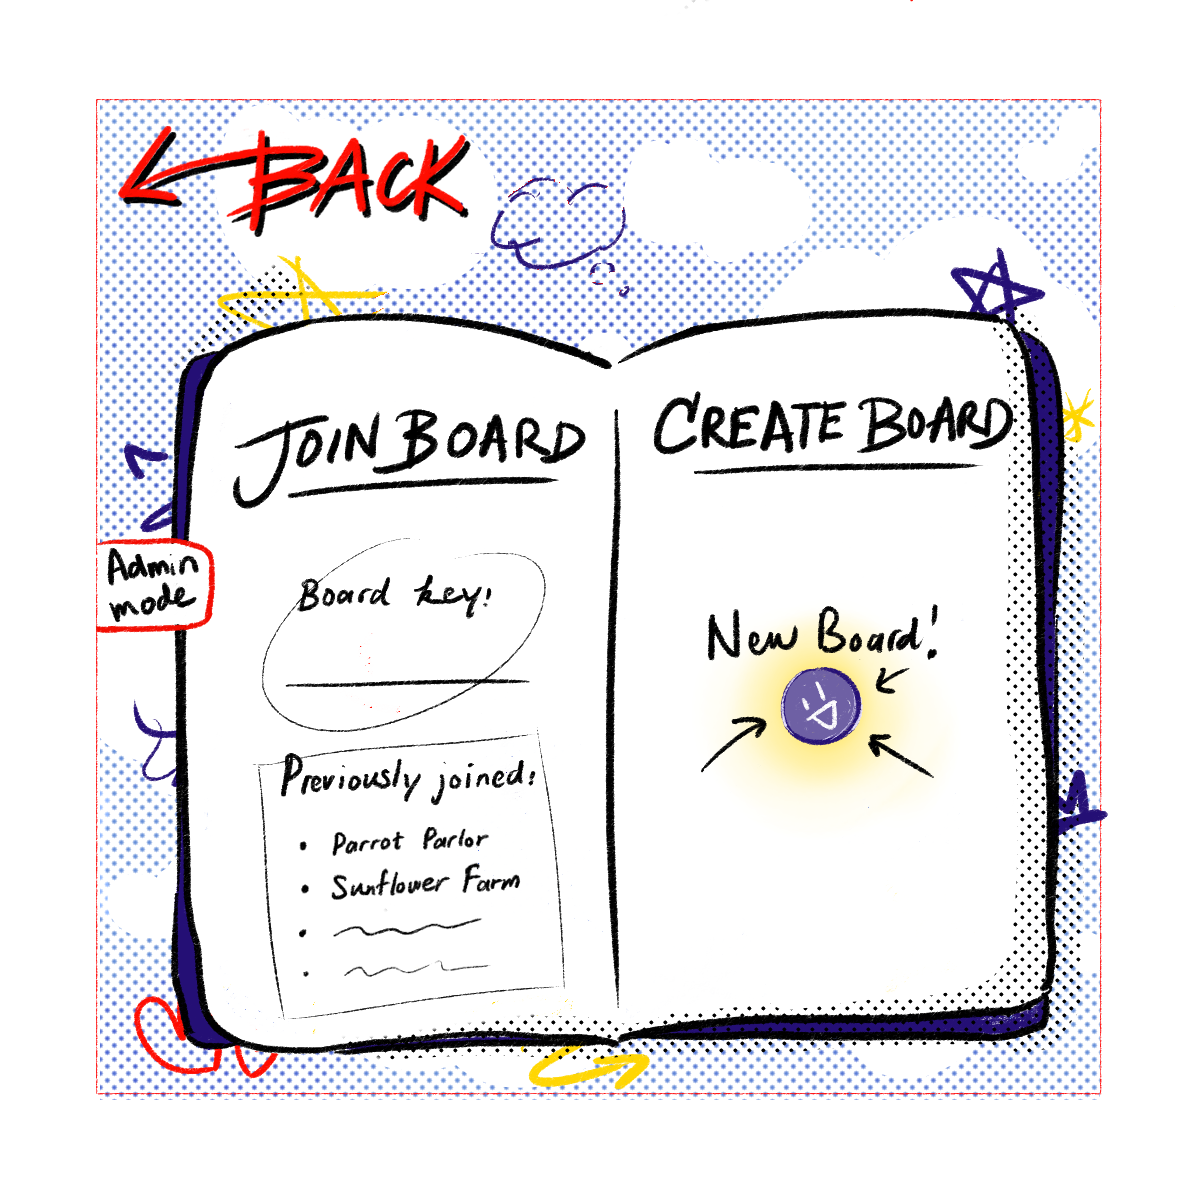
\includegraphics{mocks/hue_mock_boards.png}
    \caption{The boards screen.}
\end{figure}
\begin{figure}
    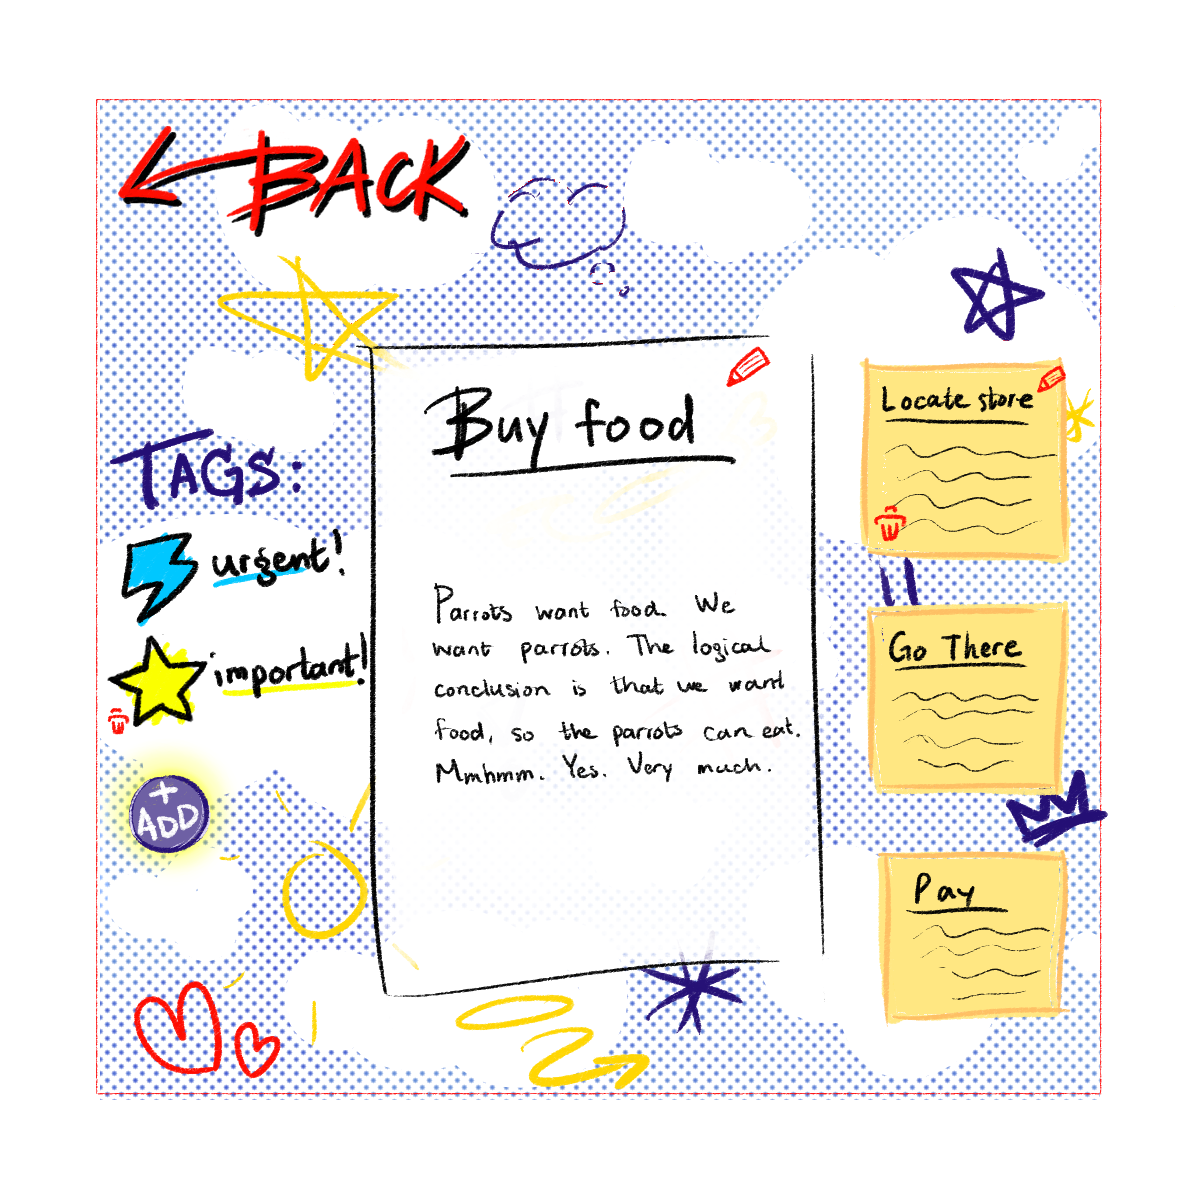
\includegraphics{mocks/hue_mock_card_details.png}
    \caption{The card details screen.}
\end{figure}